
\documentclass{beamer}
% \usetheme[secheader]{boxes}
\usecolortheme{default2}
% \usecolortheme{default}

\usepackage{lmodern}
%\usepackage[inline]{enumitem}   
% \usepackage[latin1]{inputenc}
% \usepackage{xcolor}
% \usepackage{fontenc}
\usepackage{tcolorbox}
\usepackage{latexsym}
% \usepackage{multirow}
\usepackage{amsmath,amsthm,amssymb,color}
\usepackage{array}
\usepackage{fancybox}			% For box
\usepackage{enumerate}

%---------------------------------------------------------------------------
% for \coloneqq
\usepackage{mathtools}

%---------------------------- for tikz -------------------------------------
\usepackage{tikz,tabularx}
\usetikzlibrary{decorations.pathreplacing}
\tikzstyle{every picture}+=[remember picture]
\usetikzlibrary{shapes,arrows,shadows}	
\usepgflibrary{patterns}
\usetikzlibrary{patterns}
\usetikzlibrary{shapes.geometric}
\usetikzlibrary{arrows}
\usetikzlibrary{decorations.pathreplacing}
\tikzstyle{every picture}+=[remember picture]

\setbeamertemplate{blocks}[rounded][shadow=true]

\usetikzlibrary{positioning}

\usepackage{multicol}
\setlength{\columnsep}{1cm}

\usepackage{pgfplots}
\pgfplotsset{major grid style={densely dotted,black!70}}
\pgfplotsset{compat=1.9}

%--------------------- give numbers to frames  -----------------------------
\setbeamertemplate{footline}[frame number]

%------- to remove navigation symbols at right bottom corners --------------
\setbeamertemplate{navigation symbols}{}

%-------------------------------------------
% For curved arrows
% \draw [->,red, thick] (0,0) -- (1,1) --(4,0)--(5,0) --(5,1)--(4,1);      
% \draw[->] (0,0) .. controls (1,1) .. (4,0) .. controls (5,0) and (5,1) .. (4,1);

%--------------------------- new definition shortcuts ----------------------
\def \mp {\pause}
\def \mp {}

%=================================================================

\newcommand{\ft}[1]{\frametitle{#1}}
\newcommand{\tcr}[1]{\textcolor{red}{#1}}
\newcommand{\tcb}[1]{\textcolor{blue}{#1}}
%\newcommand{\st}{\ensuremath \mathit{x}}
\newcommand{\mc}[1]{\mathcal{#1}}
\newcommand{\pr}{\mathbb{P}}
\newcommand{\sa}{\mathit{\sigma-}algebra}
\newcommand{\ninf}{n \rightarrow \infty}
\newcommand{\ninfu}{\limits_{n \rightarrow \infty}}
\newtheorem{defi}{Definition}
\newcommand{\borel}{\mathcal{B}(\mathbb{R})}
% \begin{frame}
%  \begin{figure}[t]
%   
%   \begin{tikzpicture}
%   
%   \end{tikzpicture}
% 
%   \end{figure}
% \end{frame}



\begin{document}

\begin{frame}
 
\begin{figure}[t]

    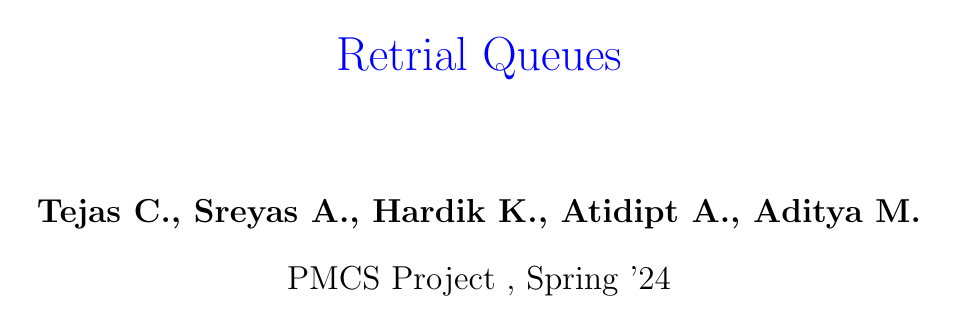
\begin{tikzpicture}


        \node [above] at (0,0.5) {\LARGE \textcolor{blue}{Retrial Queues}};


        \node [above] at (0,-1.4) {\large \textbf{Tejas C., Sreyas A., Hardik K., Atidipt A., Aditya M.}};	  

        \node [above] at (0,-2.25) {\large PMCS Project , Spring '24};


%        \node [above] at (0,-3.3-0.12) {\footnotesize PhD: IIT Bombay};	  

 %       \node [above] at (0,-3.25-0.7-0.12) {\footnotesize Post-doc:~~TIFR, LAAS-CNRS (France), University of Antwerp (Belgium), IISc};

  %      \node [above] at (0,-3.25-0.7-0.6-0.22) {\small Area of research : performance modelling, resource allocation};
        
   %     \node [above] at (0.4,-3.35-0.7-0.6-0.52) {\small queueing theory, game theory};

%         \node [above] at (0.4,-3.75-1-0.6-0.52) { (Stochastic processes)};
    \end{tikzpicture}

\end{figure}
 
\end{frame}





\begin{frame}
 \ft{Analogy}
 \begin{figure}
\includegraphics[width=10cm]{retrial}
\centering
\end{figure}
\end{frame}


\begin{frame}
 \ft{Analogy}
 \begin{figure}
\includegraphics[width=10cm]{retrial}
\centering
\end{figure}
\begin{itemize}\setlength\itemsep{.8em}
    \mp \item Busy Call Centres
    \mp \item TCP Packet Transmission
    \mp \item LAN
\end{itemize}
\end{frame}

\begin{frame}
  \ft{Notation}%\begin{figure}
% % \includegraphics[width=7cm]{renewal}
% \centering
% \end{figure}
\begin{itemize}\setlength\itemsep{.6em}
  \mp \item $\lambda:$ arrival rate of primary calls
   \mp \item $\mu:$ rate of repeated calls
    \mp \item $B(x):$ service distribution
    \mp \item $C(t):$ no of busy servers at time $t$
    \mp \item $N(t):$ no of sources of repeated calls
    \mp \item $\xi(t):$ age of current process
    \mp \item $\beta(t)=\int_{0}^{\infty}e^{-sx}dB(x):$ Laplace transform of service time
    \mp \item $b(x)=\frac{B'(x)}{1-B(x)}:$ Hazard rate
    \mp \item $k(z)=\sum_{0}^{\infty}k_nz^n=\beta(\lambda-\lambda z)$
    $$k_n=\int_{0}^{\infty}\frac{{\lambda x}^n}{n!}e^{-\lamda x}dB(x)$$
    is distribution of number of primary calls that arrive during service time of a call
 \end{itemize}


\end{frame}

\begin{frame}
\ft{M/M/1} 
\begin{itemize}\setlength\itemsep{.4em}
 \mp \item Service Time distribution \[B(x)=1-e^{-\nu x}\]
 \mp \item State transitions
 \begin{figure}
\includegraphics[width=10cm]{states}
\centering
\end{figure}
\end{itemize}
\end{frame}

\begin{frame}
\ft{M/M/1 (State Transitions)} 
    From a state $(0, n)$, only transitions into the following states are possible:
\begin{enumerate}

\item $(1, n)$ with rate $\lambda$;
\item $(1, n - 1)$ with rate $\nu$.
\end{enumerate}

Reaching state $(0, n)$ is possible only from state $(1, n)$ with rate $\nu$.

From a state $(1, n)$, only transitions into the following states are possible:
\begin{enumerate}
\item $(1, n + 1)$ with rate $\lambda$;
\item $(0, n)$ with rate $\nu$.
\end{enumerate}

Reaching state $(1,n)$ is possible only from the states: \\

  \begin{enumerate}
    \item $(0,n)$ with rate $\lambda$; 
    \item $(0,n+1)$ with rate $(n+1)\mu$; 
    \item $(1, n-1)$ with rate $\lambda$.
  \end{enumerate}
\end{frame}

\begin{frame}
\ft{M/M/1 (Limiting Distribution)} 
%  \begin{figure}
% \includegraphics[width=4cm]{hitch}
% \centering
% \end{figure}
The statistical probability equations are given by
\mp
\begin{tcolorbox}
\tcb{\[(\lambda+n\mu)p_{0n}=\nu p_{1n},\]
  \[(\lambda+\nu)p_{1n}=\lambda p_{0n}+(n+1)\mu p_{0,n+1}+\lambda p_{1,n-1} \]} 
\end{tcolorbox}
\mp 
The partial generating functions are
\begin{tcolorbox}
    \[p_{0}(z)=\frac{(1-\rho)^{\frac{\lambda}{\mu}+1}}{(1-\rho z)^{\frac{\lambda}{\mu}}}.\]    
    \begin{align*}
    p_{1}(z)&=\frac{\rho}{(1-\rho z)}p_0(z)
  \end{align*}
    \end{tcolorbox}
\end{frame}


\begin{frame}
 \ft{$M/M/1$ (Performance Metrics)}

\begin{itemize}\setlength\itemsep{.6em}
 \mp \item Mean number of jobs in queue
 \mp
\begin{tcolorbox}
\tcb{\[E[N(t)] = \frac{\rho(\lambda + \rho\mu)}{(1-\rho)\mu}\]} 
\end{tcolorbox}
The stationary distribution of the number of sources of repeated calls  $q_{n}=P{N(t)=n}$ has the generating function
\[p(z)=p_{0}(z)+p_{1}(z)=(1+\rho-\rho z)(\frac{1-\rho}{1-\rho z})^{\frac{\lambda}{\mu}+1}.\] \\ 
\[E[N(t)]=\sum np_n= p'(1)\]
\end{itemize}
\end{frame}

\begin{frame}
 \ft{$M/M/1$ (Performance Metrics)}

\begin{itemize}\setlength\itemsep{.6em}
 \mp \item Mean number of jobs in system
 \mp
\begin{tcolorbox}
\tcb{\[E[K(t)] = \frac{\rho(\lambda + \mu)}{(1-\rho)\mu}\]} 
\end{tcolorbox}
$$Q(z)=p_{0}(z)+zp_{1}(z)=(\frac{1-\rho}{1-\rho z})^{\frac{\lambda}{\mu}+1}$$.
$$E[K(t)]=Q'(1)$$
\end{itemize}
\end{frame}

\begin{frame}
 \ft{$M/M/1$ (Performance Metrics)}

\begin{itemize}\setlength\itemsep{.6em}
 \mp \item  Blocking probability
 \mp
\begin{tcolorbox}
\tcb{\[p_b = \rho = \frac{\lambda}{\nu}\]} 
\end{tcolorbox}
$P(\text{Server busy})=\sum_{n} p_{1n}= p_(1)$
\end{itemize}
\end{frame}

\begin{frame}
 \ft{$M/M/1$ (Performance Metrics)}

\begin{itemize}\setlength\itemsep{.6em}
 \mp \item  Mean sojourn time
 \mp
\begin{tcolorbox}
\tcb{\[W = \frac{\rho(\lambda + \mu)}{(1-\rho)\mu\lambda}\]} 
\end{tcolorbox}
Found using Little's Law
\end{itemize}
\end{frame}


\begin{frame}
 \ft{$M/M/1$ (Performance Metrics)}

\begin{itemize}\setlength\itemsep{.6em}
 \mp \item Recurrence Conditions
 \mp
\begin{tcolorbox}
\tcb{\begin{flalign*}
        &\rho<1& \text{for positive recurrence} \\ 
        &\rho=1& \text{for null recurrence} \\ 
        &\rho>1& \text{for transience}
    \end{flalign*}} 
\end{tcolorbox}
Proved by examining mean sojourn time
\end{itemize}
\end{frame}

\begin{frame}
 \ft{$M/M/1$ (Performance Metrics)}

\begin{itemize}\setlength\itemsep{.6em}
 \mp \item Mean no of retrials per job
 \mp
\begin{tcolorbox}
\tcb{\[E[R]= \frac{\rho(\lambda + \rho\mu)}{(1-\rho)\lambda}\]} 
\end{tcolorbox}
If a job spends time $T$ inside the queue, then it retries according to a poisson process with rate $\mu T$
\[E[R|t=T]=\mu T\]
Using law of iterated expectations, 
\[E[R]=E_T[E[R|T]]\]
\[=E_T[\mu T]\]
\[=\mu E[T]\]
\end{itemize}
\end{frame}



\begin{frame}
 \ft{$M/M/1$ (Embedded DTMC)}
% \begin{figure}
% \includegraphics[width=4cm]{mgone}
% \centering
% \end{figure}
\begin{itemize}\setlength\itemsep{.6em}
\mp\item General service times do not have the memoryless property.
\mp \item Convert CTMC to an Embedded DTMC by taking $N_i=N(\eta_i)$ i.e no of calls in orbit at the time $\eta_i$ of $i^{th}$ departure. 

\begin{equation*}
N_{i}=N_{i-1}-B_{i}+\nu_{i} 
\end{equation*}
\mp \item $B_i$ is indicator for repeated calls
\mp \item $\nu_{i}$ is no of jobs that arrive during service
\begin{equation*}
\mathrm{P}\left\{\nu_{i}=n\right\}=k_n=\int_{0}^{\infty} \frac{(\lambda x)^{n}}{n !} e^{-\lambda x} d B(x) 
\end{equation*}


\end{itemize}
\end{frame}

\begin{frame}
 \ft{Embedded DTMC}
% \begin{figure}
% \includegraphics[width=4cm]{mgone}
% \centering
% \end{figure}
\begin{itemize}
\mp \item One-step transition probabilities $r_{m n}=$ $\mathrm{P}\left\{N_{i}=n \mid N_{i-1}=m\right\}$ are given by the formula


\begin{equation*}
r_{m n}=\frac{\lambda}{\lambda+m \mu} k_{n-m}+\frac{m \mu}{\lambda+m \mu} k_{n-m+1} 
\end{equation*}

\mp \item Mean Length of queue 
\[E[N]=\rho+\frac{\lambda \rho}{1-\rho}\left( \frac{1}{\mu}+\frac{1}{\nu}\right)\]

\end{itemize}
\end{frame}

\begin{frame}
 \ft{Special Case: $M/M/2$}
\begin{itemize}\setlength\itemsep{.4em}

\mp \item Consider the basic case of multi server model (Taking $\nu$=1)

\[ p_{0 j}=\mathrm{P}\{C(t)=0, N(t)=j\}\]
\[ p_{1 j}=\mathrm{P}\{C(t)=1, N(t)=j\} \]
\[p_{2 j}=\mathrm{P}\{C(t)=2, N(t)=j\}\]


be the limiting distributions. These probabilities satisfy the following statistic probability equations


\begin{align*}
(\lambda+j \mu) p_{0 j} & =p_{1 j} \\
(\lambda+1+j \mu) p_{1 j} & =\lambda p_{0 j}+(j+1) \mu p_{0, j+1}+2 p_{2 j}  \\
(\lambda+2) p_{2 j} & =\lambda p_{1 j}+(j+1) \mu p_{1, j+1}+\lambda p_{2, j-1} 
\end{align*}
and normalizing condition
\[\sum_{j=0}^{\infty}\left(p_{0 j}+p_{1 j}+p_{2 j}\right)=1 \]
\end{itemize}
\end{frame}









\begin{frame}
 \ft{Simulating $M/M/1$}
\begin{itemize}\setlength\itemsep{.8em}

\mp \item The arrival of jobs , the retrial of jobs in orbit and the processing of the jobs is simulated by generating random numbers.

\mp \item This gives us the pre-computed values of various parameters like arrival time , departure time, number of retrials etc . These will be used to compute various performence metrics.
% \mp  \item Store information(Arrival time, Scheduled time,Departure time,No of pings) about a job in a sorted set
% \mp \item Compute Service Rate(exp($\mu$)) ,and hence keep a track of the next time queue gets free.
% \mp \item The 


% \mp\item Recall that for an $M/M/1$ queue, $1-\pi(0) = \frac{\lambda}{\mu} = \lambda b$.

\end{itemize}
\end{frame}
\begin{frame}
 \ft{Simulating $M/M/1$}
\begin{itemize}\setlength\itemsep{.8em}

% \section{Simulations}

% Parameters: $\lambda = 5, \vu = 7,\mu =1 $
% \begin{center}
    
% \begin{tabular}{c|c|c|}
%      Parameter&Expected Values&Simulated Values  \\
%     Mean Sojourn Time&3&3.16 \\
%     Blocking Probability&0.71 &0.705 \\
%     Mean No of jobs&15&15.85\\
%     Mean No of pings&3&3.02\\
%     % & & \\
% \end{tabular}
Parameters:$\lambda=5, \nu=7, \mu=1$
\begin{table}[htbp]
    \centering
    \begin{tabular}{|c|c|c|}
        \hline
        Parameter & Expected Values & Simulated Values  \\
        \hline
        Mean Sojourn Time & 3 & 3.16 \\
        Blocking Probability & 0.71 & 0.705 \\
        Mean No of jobs & 15 & 15.85 \\
        Mean No of pings & 3 & 3.02 \\
        \hline
    \end{tabular}
\end{table}

\end{itemize}
\end{frame}


\begin{frame}
% ARRIVAL TIMES
\begin{figure}
    \centering
    \includegraphics[width=0.75\linewidth]{images/arrival_times.png}
    \caption{Arrival Times of the Jobs}
    \label{Arrival Times of the Jobs}
    \\
The arrival times increase linearly with time.\\
\end{figure}
\end{frame}

% INTERARRIVAL TIMES
\begin{frame}
\begin{figure}
    \centering
    \includegraphics[width=0.75\linewidth]{images/interarrival1.png}
    \caption{Interarrival Times}
    \label{Arrival Times of the Jobs}
\end{figure}
\end{frame}

\begin{frame}
\begin{figure}
    \centering
    \includegraphics[width=0.75\linewidth]{images/interarrival2.png}
    \caption{Interarrival Times}
    \label{InterArrival Times of the Processes}
    \\
Clearly, the interarrival times are independent of eachother.\\
\end{figure}
\end{frame}

% INTERARRIVAL TIMES
\begin{frame}
\begin{figure}
    \centering
    \includegraphics[width=0.75\linewidth]{images/interarrival1.png}
    \caption{Interarrival Times}
    \label{Arrival Times of the Jobs}
\end{figure}
\begin{figure}
    \centering
    \includegraphics[width=0.75\linewidth]{images/interarrival2.png}
    \caption{Your Image Caption}
    \label{InterArrival Times of the Processes}
    \\
Clearly, the interarrival times are independent of eachother.\\
\end{figure}
\end{frame}

\begin{frame}
% VERIFICATION OF LITTLE LAW
\begin{figure}
    \centering
    \includegraphics[width=0.75\linewidth]{images/littles_law_verification.png}
    \caption{Verification of Little's Law}
    \label{E[N]/E[T] vs N}
Little's Law is verified by:
$$ E[N]/E[T]$$
converges to $\lambda$ \\
\end{figure}

\end{frame}
% BLOCKING PROBABILITY
\begin{figure}
    \centering
    \includegraphics[width=0.75\linewidth]{images/blocking_probability.png}
    \caption{Blocking Probability vs Number of Jobs arrived(N)}
    \label{Blocking Probability vs N}
\\
The Blocking Probability stagnates to 0.70.
\end{figure}
\end{document} 
